\documentclass{article}

\author{Teddy Krulewich}
\title{\vspace{-4em}HW4 ME5501 – Robotics and Unmanned Systems}

\usepackage{graphicx}
\graphicspath{ {images/} }


\usepackage[utf8]{inputenc}
\usepackage{minted}
\usepackage{hyperref}
\usepackage{xcolor}
\definecolor{bg}{rgb}{0.95,0.95,0.95}
\usepackage{caption}
\usepackage{mdframed}

\begin{document}
\maketitle

\section*{Problem 1}
Complete the following ROS tutorials at \url{https://docs.ros.org/en/foxy/Tutorials.html}

• Understanding ROS Nodes

• Understanding ROS Topics

\bigskip
\noindent Save a screenshot of the Turtlebot simulator and show/print the screenshot.


\begin{figure}[H]
  \centering
  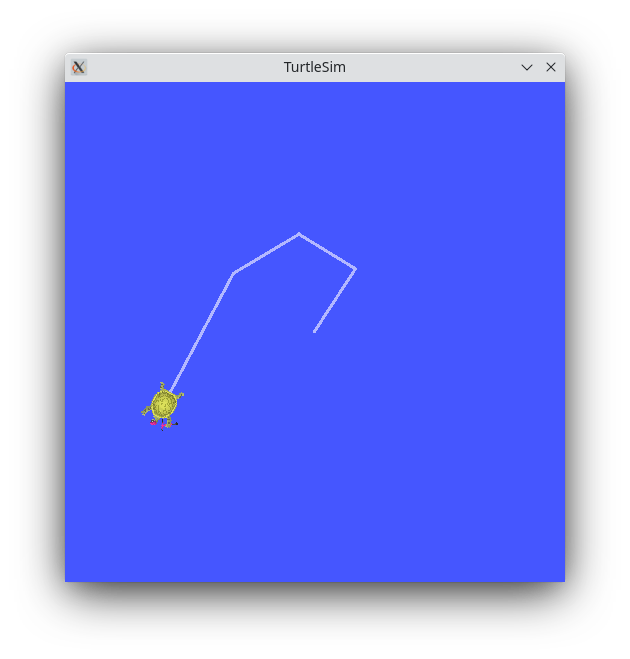
\includegraphics[width=0.5\textwidth]{question1.png}
  \caption*{Screenshot of Turtlebot Simulator}
\end{figure}

\section*{Problem 2}

Complete the following ROS tutorials at

\url{http://wiki.ros.org/ROS/Tutorials}


• 12. Writing a Simple Publisher and Subscriber (Python) 


• 13. Examining the Simple Publisher and Subscriber 

\bigskip 
\noindent Save a screenshot of the running code in tutorials 13, and print these screenshots to turn in.

\begin{figure}[H]
  \centering
  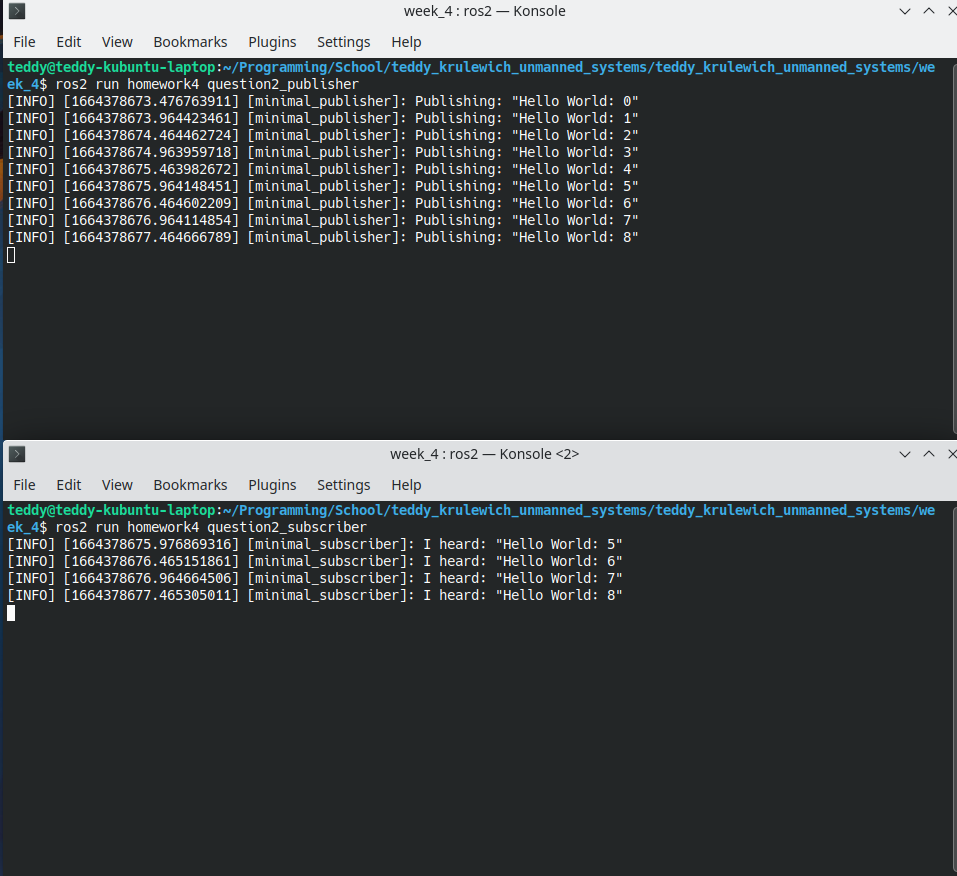
\includegraphics[width=\textwidth]{question2.png}
  \caption*{Screenshot of subscriber and publisher running}
\end{figure}

\bigskip
\section*{Problem 3}

For this problem you will be using ROS2 and Gazebo to simulate the Turtlebot3 Burger platform.  
Help in loading the simulation can be found at 
\url{http://emanual.robotis.com/docs/en/platform/turtlebot3/simulation/}.

\bigskip
\noindent Make sure to go to the Gazebo part of the E-manual. When setting the model type, replace “\$\{TB3\_MODEL\}” with 
“burger.” 

\bigskip
\noindent Create a ROS2 node that makes the Turtlebot3 travel forward at 1.5 m/s (remember this speed is 
much faster than it can do in real life) for 5 seconds, then turns to the right at 0.15 rad/s for 2 
seconds, then continues forward at 1.5 m/s for another 5 seconds before stopping. Log the position 
data, and velocity \& angular velocity commands.

\bigskip 
\noindent Create a subplot of the x \& y position data, velocity \& angular velocity commands versus time. 

\bigskip
\noindent Submit your Python code.

\begin{figure}[H]
  \centering
  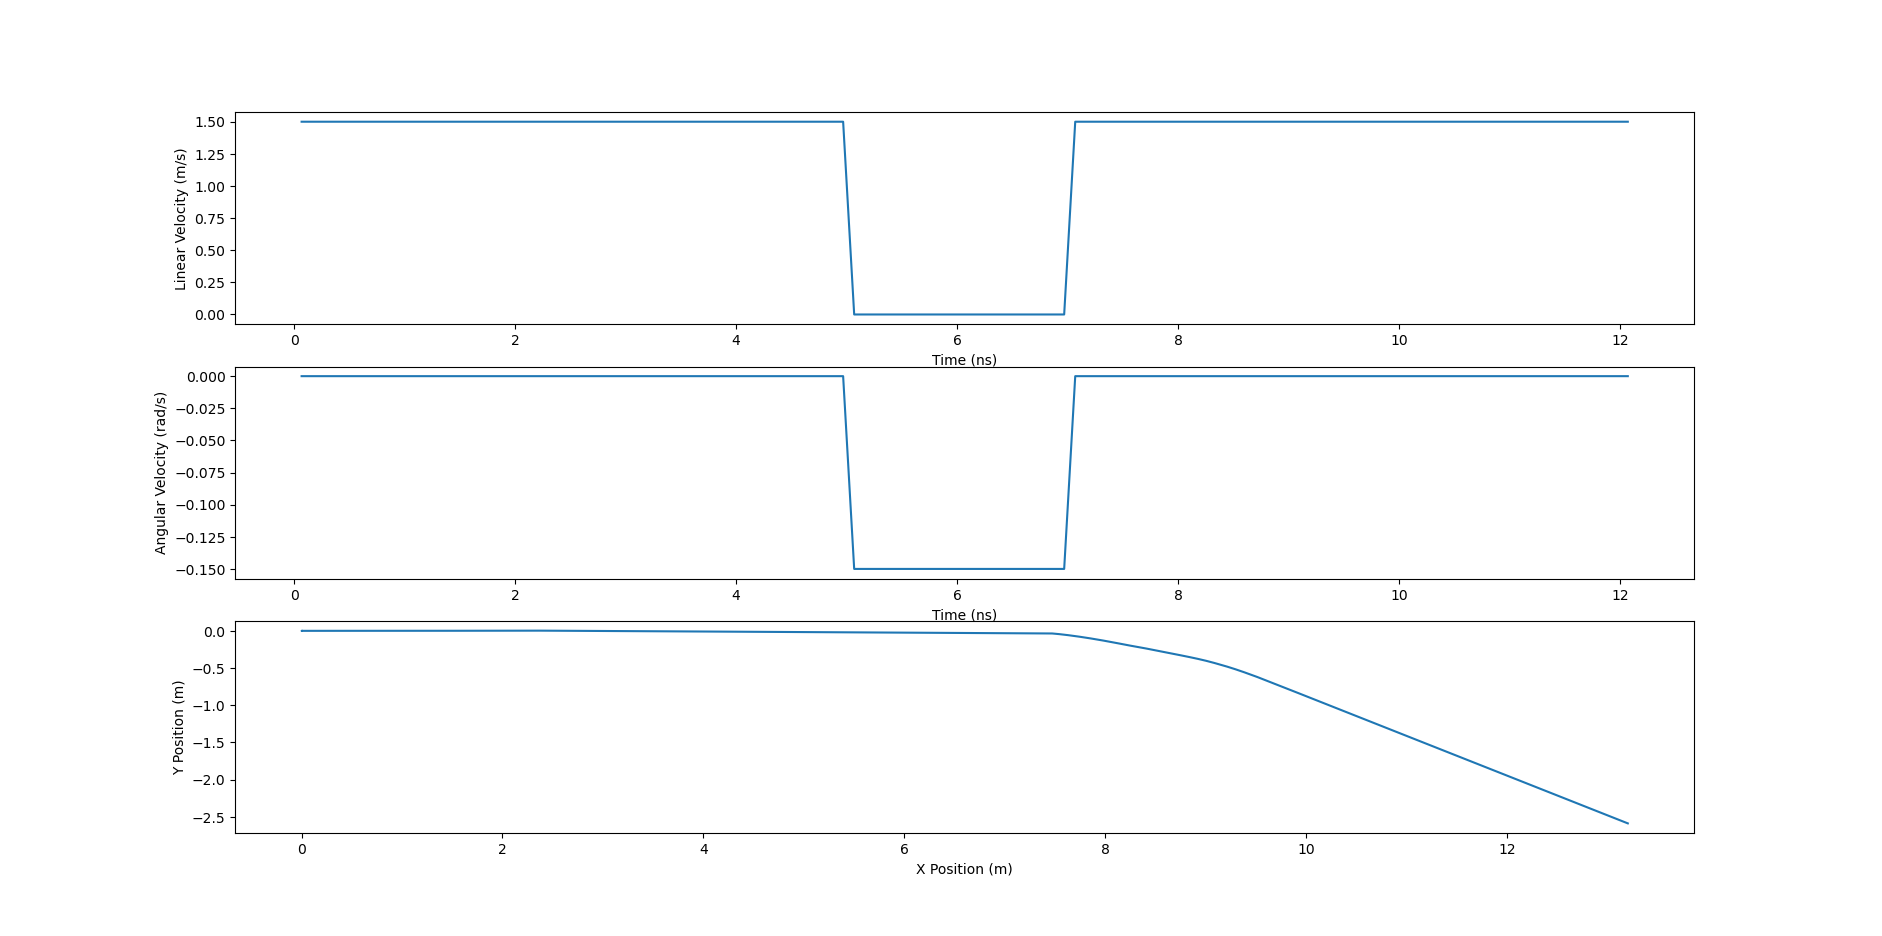
\includegraphics[width=\textwidth]{question3.png}
  \caption*{Plot of position data, velocity, and angular velocity commands versus time}
\end{figure}

\begin{minted}[bgcolor=bg,fontsize=\footnotesize,linenos]{python}
import rclpy
from rclpy.node import Node

from geometry_msgs.msg import Twist
from nav_msgs.msg import Odometry

import matplotlib.pyplot as plt
import numpy as np
import math

def euler_from_quaternion(x:float, y:float, z:float, w:float) -> tuple:
  """
  Convert a quaternion into euler angles (roll, pitch, yaw)
  roll is rotation around x in radians (counterclockwise)
  pitch is rotation around y in radians (counterclockwise)
  yaw is rotation around z in radians (counterclockwise)
  """
  t0 = +2.0 * (w * x + y * z)
  t1 = +1.0 - 2.0 * (x * x + y * y)
  roll_x = math.atan2(t0, t1)
   
  t2 = +2.0 * (w * y - z * x)
  t2 = +1.0 if t2 > +1.0 else t2
  t2 = -1.0 if t2 < -1.0 else t2
  pitch_y = math.asin(t2)
   
  t3 = +2.0 * (w * z + x * y)
  t4 = +1.0 - 2.0 * (y * y + z * z)
  yaw_z = math.atan2(t3, t4)
   
  return roll_x, pitch_y, yaw_z # in radians


class TurtleBotController(Node):
  # A commanded foward and rotation velocity for the turtlebot with
  #  a specified duration
  class VelocityCommand:
  def __init__(self, linear, angular, duration):
  self.twist = Twist()
  self.twist.linear.x = linear
  self.twist.angular.z = angular
  self.duration = duration

  def __init__(self):
  super().__init__('turtlebot_controller')

  # create a publisher to send velocity commands to the turtlebot
  self.cmd_vel_publisher = self.create_publisher(Twist, 'cmd_vel', 10)
  # create a subscriber to read sensor data
  self.odom_subscriber = self.create_subscription(Odometry, 'odom', 
  self.odom_callback, 10)

  # will store a list of commands to execute
  self.velocity_commands = []

  # store the time the node was started
  self.start_time = self.get_clock().now().nanoseconds
  self.time_command_started = self.start_time

  # when all commands are executed will be true
  self.done = False

  # tracks the state of commands, position, and angle over time
  self.state_records = { 'cmd_vel_linear': [], 'cmd_vel_angular': [], 
  'x': [], 'y': [], 'theta': [] }


  
  def add_move_command(self, linear, angular, duration):
  self.velocity_commands.append(
  TurtleBotController.VelocityCommand(linear, angular, duration))
  
  def odom_callback(self, msg):
  time = self.get_clock().now().nanoseconds
  # the total time elapsed since the node started
  time_elapsed_total = time - self.start_time

  # the time elapsed while executing current command
  time_elapsed_command = time - self.time_command_started

  # store current sensor data for logging and plotting
  self.state_records['x'].append(
  (time_elapsed_total, msg.pose.pose.position.x))

  self.state_records['y'].append(
  (time_elapsed_total, msg.pose.pose.position.y))

  theta = euler_from_quaternion(
  msg.pose.pose.orientation.x,
  msg.pose.pose.orientation.y,
  msg.pose.pose.orientation.z,
  msg.pose.pose.orientation.w)[2]
  
  self.state_records['theta'].append((time_elapsed_total, theta))

  # if we have not finished executing commands
  if len(self.velocity_commands) > 0:
  # if the current command has executed for the specified duration
  # then move on to the next command
  if time_elapsed_command >= self.velocity_commands[0].duration:
  self.velocity_commands.pop(0)
  self.time_command_started = self.get_clock().now().nanoseconds

  # if there are no remaining commands we are done!
  if len(self.velocity_commands) == 0:
    # publishes an empty Twist velocity causing the 
    # turtlebot to stop moving
    self.cmd_vel_publisher.publish(Twist())
    self.get_logger().info('No more commands')

    self.done = True
    return
  
  # store the current command velocities for logging and plotting
  self.state_records['cmd_vel_linear'].append(
  (time_elapsed_total, self.velocity_commands[0].twist.linear.x))
  
  self.state_records['cmd_vel_angular'].append(
  (time_elapsed_total, self.velocity_commands[0].twist.angular.z))
  
  # publish the velocity command to the turtle bot
  self.cmd_vel_publisher.publish(self.velocity_commands[0].twist)

def main(args=None):
  rclpy.init(args=args)

  # create a turtlebot
  turtlebot_controller = TurtleBotController()

  # command the turtlebot to move forward at 1.5 m/s for 5 seconds
  turtlebot_controller.add_move_command(1.5, 0.0, 5000000000)
  # then comand the turtlebot to turn at 0.15 rad/s for 2 seconds
  turtlebot_controller.add_move_command(0.0, -0.15, 2000000000)
  # then command the turtle bot to move forward at 1.5 m/s for 5 seconds
  turtlebot_controller.add_move_command(1.5, 0.0, 5000000000)

  # while the turtle bot hasn't finsihed executing its commands, update the node
  while not turtlebot_controller.done:
  rclpy.spin_once(turtlebot_controller)
  
  
  fig, ax = plt.subplots(3, 1)

  # plot the linear velocity command vs time
  ax[0].plot([x[0] / 1000000000 for x in
  turtlebot_controller.state_records['cmd_vel_linear']], 
  [x[1] for x in turtlebot_controller.state_records['cmd_vel_linear']],
  label='linear')

  ax[0].set_xlabel('Time (ns)')
  ax[0].set_ylabel('Linear Velocity (m/s)')

  # plot the angular velocity command vs time
  ax[1].plot([x[0] / 1000000000 for x in 
  turtlebot_controller.state_records['cmd_vel_angular']],
  [x[1] for x in turtlebot_controller.state_records['cmd_vel_angular']],
  label='angular')

  ax[1].set_xlabel('Time (ns)')
  ax[1].set_ylabel('Angular Velocity (rad/s)')

  # plot the x and y position of the turtlebot, showing the path
  ax[2].plot([x[1] for x in turtlebot_controller.state_records['x']], 
  [y[1] for y in turtlebot_controller.state_records['y']], label='y')
  
  ax[2].set_xlabel('X Position (m)')
  ax[2].set_ylabel('Y Position (m)')
  

  plt.show()
  

  turtlebot_controller.destroy_node()
  rclpy.shutdown()


if __name__ == '__main__':
  main()

\end{minted}

\section*{Problem 4}
Create a ROS2 node/script that uses a feedback controller to control the heading of the Turtlebot3. 
Once you have adequately tuned the controller, collect the data (by writing to a log file) from a 90 
degree step input (use a forward speed of 0.15 m/s).

\bigskip
\noindent Create a plot of the desired and actual heading versus time. What is the rise time, settling time, and 
percent overshoot of your controller? 

\bigskip
\noindent Submit your Python code.

\begin{figure}[H]
  \centering
  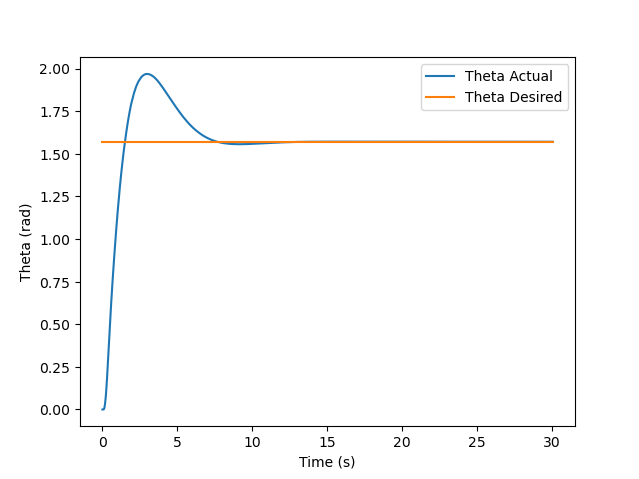
\includegraphics[width=\textwidth]{question4.png}
  \caption*{Plot of desired and actual heading versus time}
\end{figure}

\noindent The rise time was 0.70 - 0.2191 = \textbf{0.4809 seconds.} 

\noindent The settling time was 1.3 - 0.8042 =  \textbf{0.4958 seconds.} 

\noindent The percent overshoot was 100 * (91.855 / 90.0 - 1.0) = \textbf{2.06\%}.

\bigskip
\noindent \textbf{I updated the previous code in Problem 2 by adding a PID controller}



\begin{minted}[bgcolor=bg,fontsize=\footnotesize,linenos]{python}
class PID:
  """
  Simple PID controller for a single variable
  """
  def __init__(self, kp, ki, kd):
  self.kp = kp
  self.ki = ki
  self.kd = kd

  self.last_error = 0
  self.integral = 0

  self.output = 0

  def update(self, error, dt):
  """
  Update the PID controller using new error value
  """
  self.integral += error * dt
  derivative = (error - self.last_error) / dt

  self.output = self.kp * error + self.ki * self.integral + self.kd * derivative

  self.last_error = error
\end{minted}

\noindent \textbf{I modified the constuctor adding the following}

\begin{minted}[bgcolor=bg,fontsize=\footnotesize,linenos]{python}
class TurtleBotController(Node):
  def __init__(self):
  super().__init__('turtlebot_controller')
  ...
  ...
  # used to calculate dt between updates
  self.last_update = self.start_time

  # desried heading
  self.desired_theta = None
  self.current_theta = None

  self.theta_controller = PID(1, 0.5, 0.0)
\end{minted}

\noindent \textbf{I modified the callback function as follows}

\begin{minted}[bgcolor=bg,fontsize=\footnotesize,linenos]{python}
def odom_callback(self, msg):
  # if we are done dont execute anything else
  if self.done:
  return

  # if we have not set a desired heading 
  if self.desired_theta is None:
  self.done = True
  
  # get current time and time elapsed since the node was started
  time = self.get_clock().now().nanoseconds
  time_elapsed = time - self.start_time

  # get the dt in seconds since the last update
  dt = (time - self.last_update)
  

  # read sensor data to get position and heading
  self.current_x = msg.pose.pose.position.x
  self.current_y = msg.pose.pose.position.y
  self.current_theta = euler_from_quaternion(
  msg.pose.pose.orientation.x,
  msg.pose.pose.orientation.y, 
  msg.pose.pose.orientation.z,
  msg.pose.pose.orientation.w)[2]

  # store sensor data for logging and plotting
  self.state_records['x'].append((time_elapsed, self.current_x))
  self.state_records['y'].append((time_elapsed, self.current_y))
  self.state_records['theta'].append((time_elapsed, self.current_theta))

  # create a Twist for the velocity command
  twist = Twist()
  # move forward at 0.15 m/s
  twist.linear.x = 0.15


  # if more than 3 seconds have elapsed, stop the turtlebot
  if time_elapsed > 3000000000: 
  twist.angular.z = 0.0
  self.cmd_vel_publisher.publish(twist)
  self.done = True
  return
  
  # run a PID controller using the error in heading
  self.theta_controller.update(self.desired_theta - self.current_theta, dt)
  
  # set the angular velocity to the output of the PID controller
  twist.angular.z = self.theta_controller.output

  twist.angular.z = clamp(twist.angular.z, -2.84, 2.84)

  # publish the velocity command to the turtlebot
  self.cmd_vel_publisher.publish(twist)

  # store the velocity command for logging and plotting
  self.state_records['cmd_vel_linear'].append((time, twist.linear.x))
  self.state_records['cmd_vel_angular'].append((time, twist.angular.z))

  self.last_update = time
\end{minted}

\noindent \textbf{I modified the main function as follows}

\begin{minted}[bgcolor=bg,fontsize=\footnotesize,linenos]{python}
def main(args=None):
  rclpy.init(args=args)

  turtlebot_controller = TurtleBotController()

  turtlebot_controller.desired_theta = math.pi / 2

  while not turtlebot_controller.done:
    rclpy.spin_once(turtlebot_controller)
  ...
  ...
\end{minted}

\end{document}